\chapter{Orientamenti politici delle principali testate giornalistiche mondiali}
\label{chap:orientamenti_press}

\section{Introduzione}
In questo capitolo vengono analizzati gli orientamenti politici delle principali testate giornalistiche mondiali. Il quadro editoriale internazionale si distingue in diverse macro-aree — neutrali, centro-sinistra, centro, centro-destra, e cattolico-centrista — ottenute attraverso esercitazioni universitarie, analisi testuali quantitative e \gls{survey-internazionali}.

\section{Classificazione delle testate}
Di seguito la classificazione delle principali testate mondiali in base al loro orientamento politico:

\begin{table}[h]
  \centering
  \begin{tabular}{|p{5cm}|p{10cm}|}
    \hline
    \textbf{Orientamento politico} & \textbf{Testate} \\
    \hline
    Neutrali / Indipendenti & The Guardian \cite{theguardian}, BBC News \cite{bbcnews}, Reuters \cite{reuters}, Al Jazeera \cite{aljazeera}, The New York Times \cite{thenewyorktimes}, Dawn \cite{dawn} \\
    \hline
    Centro-sinistra / Progressisti & The Washington Post \cite{thewashingtonpost}, Le Monde \cite{lemonde}, La Repubblica \cite{larepubblica}, CNN \cite{cnn}, Folha de S.Paulo \cite{folhadespaulo}, The Hindu \cite{thehindu}, Globe and Mail \cite{globeandmail}, Financial Times \cite{financialtimes}, El País \cite{elpais}, Der Spiegel \cite{derspiegel}, Süddeutsche Zeitung \cite{suddeutschezeitung}, China Daily \cite{chinadaily}, Asahi Shimbun \cite{asahishimbun} \\
    \hline
    Centro-destra / Conservatori & Corriere della Sera \cite{corrieredellasera}, The Straits Times \cite{thestraitstimes}, Bloomberg News \cite{bloombergnews}, Clarín \cite{clarín}, The Korea Times \cite{thekoreatimes}, The Wall Street Journal \cite{thewallstreetjournal} \\
    \hline
  \end{tabular}
  \caption{Classificazione delle testate giornalistiche mondiali per orientamento politico.}
  \label{tab:classificazione_testate}
\end{table}

\begin{figure}
    \centering
    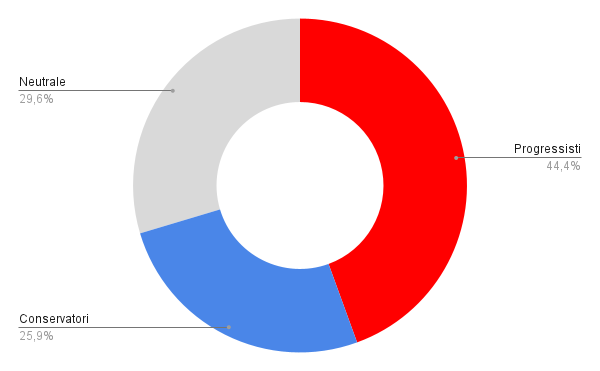
\includegraphics[width=0.75\linewidth]{Immagini/Classificazione delle Testate.png}
    \caption{Suddivisione delle testate giornalistiche utilizzate per l'analisi}
    \label{fig:enter-label}
\end{figure}

\section{Metodologia di classificazione}
Il metodo utilizzato per la classificazione delle testate giornalistiche oggetto della nostra analisi si articola in tre principali fasi. In primo luogo, è stato condotto uno studio della storia di ciascuna testata, in modo tale da comprenderne l’evoluzione editoriale, le linee guida ideologiche nel tempo, ed il contesto socio-politico in cui si è sviluppata. Successivamente, è stata effettuata una ricerca online finalizzata alla raccolta di informazioni aggiornate e pertinenti per ottenere un quadro il più possibile completo ed obiettivo. Infine, tale materiale è stato integrato con una valutazione personale elaborata a partire dalle nostre osservazioni critiche, esperienze dirette di lettura e riflessioni maturate nel corso del progetto. \\ 
Questo approccio, pur riconoscendo una componente soggettiva, mira ad offrire una classificazione ragionata e consapevole, fondata su una pluralità di prospettive e su un'analisi documentata.
